\documentclass[french]{amu_these}

\begin{document}

										
	\chead{}
\pdfbookmark[0]{Page de titre}{titre}
\thispagestyle{empty}
\newgeometry{margin=2em}
% \newgeometry{left=3em,right=2em,top=2em,bottom=2em} %% marge pour la reliure en cas d'exemplaire imprimé

\begin{center}
	\begin{minipage}[c]{.5\linewidth}
		\raggedright
\includegraphics[height=7em]{logo_amu}
	\end{minipage}\hfill
	\begin{minipage}[c]{.5\linewidth}
		%\raggedleft\includegraphics[height=7em]{example-image-b} %% logo établissement en cotutelle, le cas échéant
	\end{minipage}\hfill
\end{center}

\vspace{1em}

\begin{center}
	\begin{minipage}[c]{.77\linewidth}
		\dhorline{\textwidth}{4pt}
	\end{minipage}\hfill
	\begin{minipage}[c]{.23\linewidth}
		\raggedleft\titl{NNT : 2023AIXM0001}
		% renseigner votre numéro national de thèse (NNT)
	\end{minipage}\hfill
\end{center}

%\vspace{1em}

\doublespacing
\begin{flushleft}
    \titb{\HUGE\textcolor{cyanamu}{THÈSE DE DOCTORAT}}\\
	\titl{\Large Soutenue à Aix-Marseille Université}\\
	%\titl{\Large dans le cadre d'une cotutelle avec }\\ %% établissement en cotutelle, le cas échéant
	\titl{\Large le 10 janvier 2023 par}\\
\end{flushleft}
\vspace{2em}
\begin{center}
	\titsb{\Huge Prénom NOM}\\
    \vspace{1em}
	\titm{\LARGE Titre de la thèse:}\\ 
 	\titm{\Large sous-titre de la thèse}\\
\end{center}
\singlespacing

\vspace{4em}

\begin{center}
	\begin{minipage}[t]{.45\linewidth}
    	    \vspace{.5em}
        	\titb{Discipline}
        	
        	\titl{Voir la liste des disciplines en \hyperref[chap:doctorats]{annexe A}}
        	
    	    \vspace{1em}
        	\titb{Spécialité}
        	
        	\titl{Voir la liste des spécialités en \hyperref[chap:doctorats]{Annexe A}}
        	
    	    \vspace{2em}
        	\titb{École doctorale}
        	
        	\titl{Voir la liste des écoles doctorales en \hyperref[chap:doctorats]{Annexe A}}
        	
    	    \vspace{1em}
        	\titb{Laboratoire/Partenaires de recherche}
        	
        	\titl{Renseigner les partenaires institutionnels\\
        	et les partenaires privés, un partenaire par ligne
        	}

    	    \vspace{3em}
        	\titl{Pour les consignes de présentation détaillées\\
			des pages liminaires, voir en \hyperref[chap:consignes]{Annexe B}}
	\end{minipage}\hfill
	\begin{minipage}[t]{.03\linewidth}
	    \dvertline{4pt}{-24em}
	\end{minipage}\hfill
	\begin{minipage}[t]{.52\linewidth}
	    \vspace{.5em}
    	\titb{\small Composition du jury}

	    \vspace{1em}
    	\titl{
        \begin{tabular}{p{12em} p{9.5em}}
        	Prénom NOM & Rapporteur·e \\
        	Titre et affiliation \\
        	\\
        	Prénom NOM & Rapporteur·e \\
        	Titre et affiliation \\
            \\
            Prénom NOM & Examinateur·rice \\
        	Titre et affiliation \\
            \\
        	Prénom NOM & Président·e du jury \\
        	Titre et affiliation \\
            \\
        	Prénom NOM & Directeur·rice de thèse \\
        	Titre et affiliation \\
           \\
        	Prénom NOM & Membre invité·e \\
        	Titre et affiliation \\
        \end{tabular}
        }
	\end{minipage}\hfill
\end{center}       

\vspace{2em}

\begin{center} %% logos partenaires
	\begin{minipage}[c]{.25\linewidth}
		\centering\includegraphics[height=5em]{example-image-a} 
	\end{minipage}\hfill
	\begin{minipage}[c]{.25\linewidth}
		\centering\includegraphics[height=5em]{example-image-b}
	\end{minipage}\hfill
	\begin{minipage}[c]{.25\linewidth}
		\centering\includegraphics[height=5em]{example-image-c} 
	\end{minipage}\hfill
	\begin{minipage}[c]{.25\linewidth}
		\centering\includegraphics[height=5em]{example-image-c}
	\end{minipage}\hfill
\end{center}

\restoregeometry
				%% page de titre
										
	\newpage
\addchap{Affidavit}
\label{chap:affidavit}
\thispagestyle{empty}

\iftrue % Déclaration sur l'honneur pour une thèse en français (inverser les \if pour une thèse en anglais)
    Je soussigné, [Prénom Nom], %% Prénom et Nom de l'auteur %%
    déclare par la présente que le travail présenté dans ce manuscrit est mon propre travail, réalisé sous la direction scientifique de [Prénom Nom], % Prénom et Nom du directeur de thèse et s’il y a lieu du co-directeur de thèse
    dans le respect des principes d’honnêteté, d'intégrité et de responsabilité inhérents à la mission de recherche. Les travaux de recherche et la rédaction de ce manuscrit ont été réalisés dans le respect à la fois de la charte nationale de déontologie des métiers de la recherche et de la charte d’Aix-Marseille Université relative à la lutte contre le plagiat.
    
    Ce travail n'a pas été précédemment soumis en France ou à l'étranger dans une version identique ou similaire à un organisme examinateur.\\
    
    Fait à [ville] le [date]
    
    \begin{flushright}\includegraphics[width=120px,height=40px]{example-image-a}\end{flushright}% signature

    ~\vfill
    \begin{center}
        \begin{minipage}[c]{0.25\linewidth}
            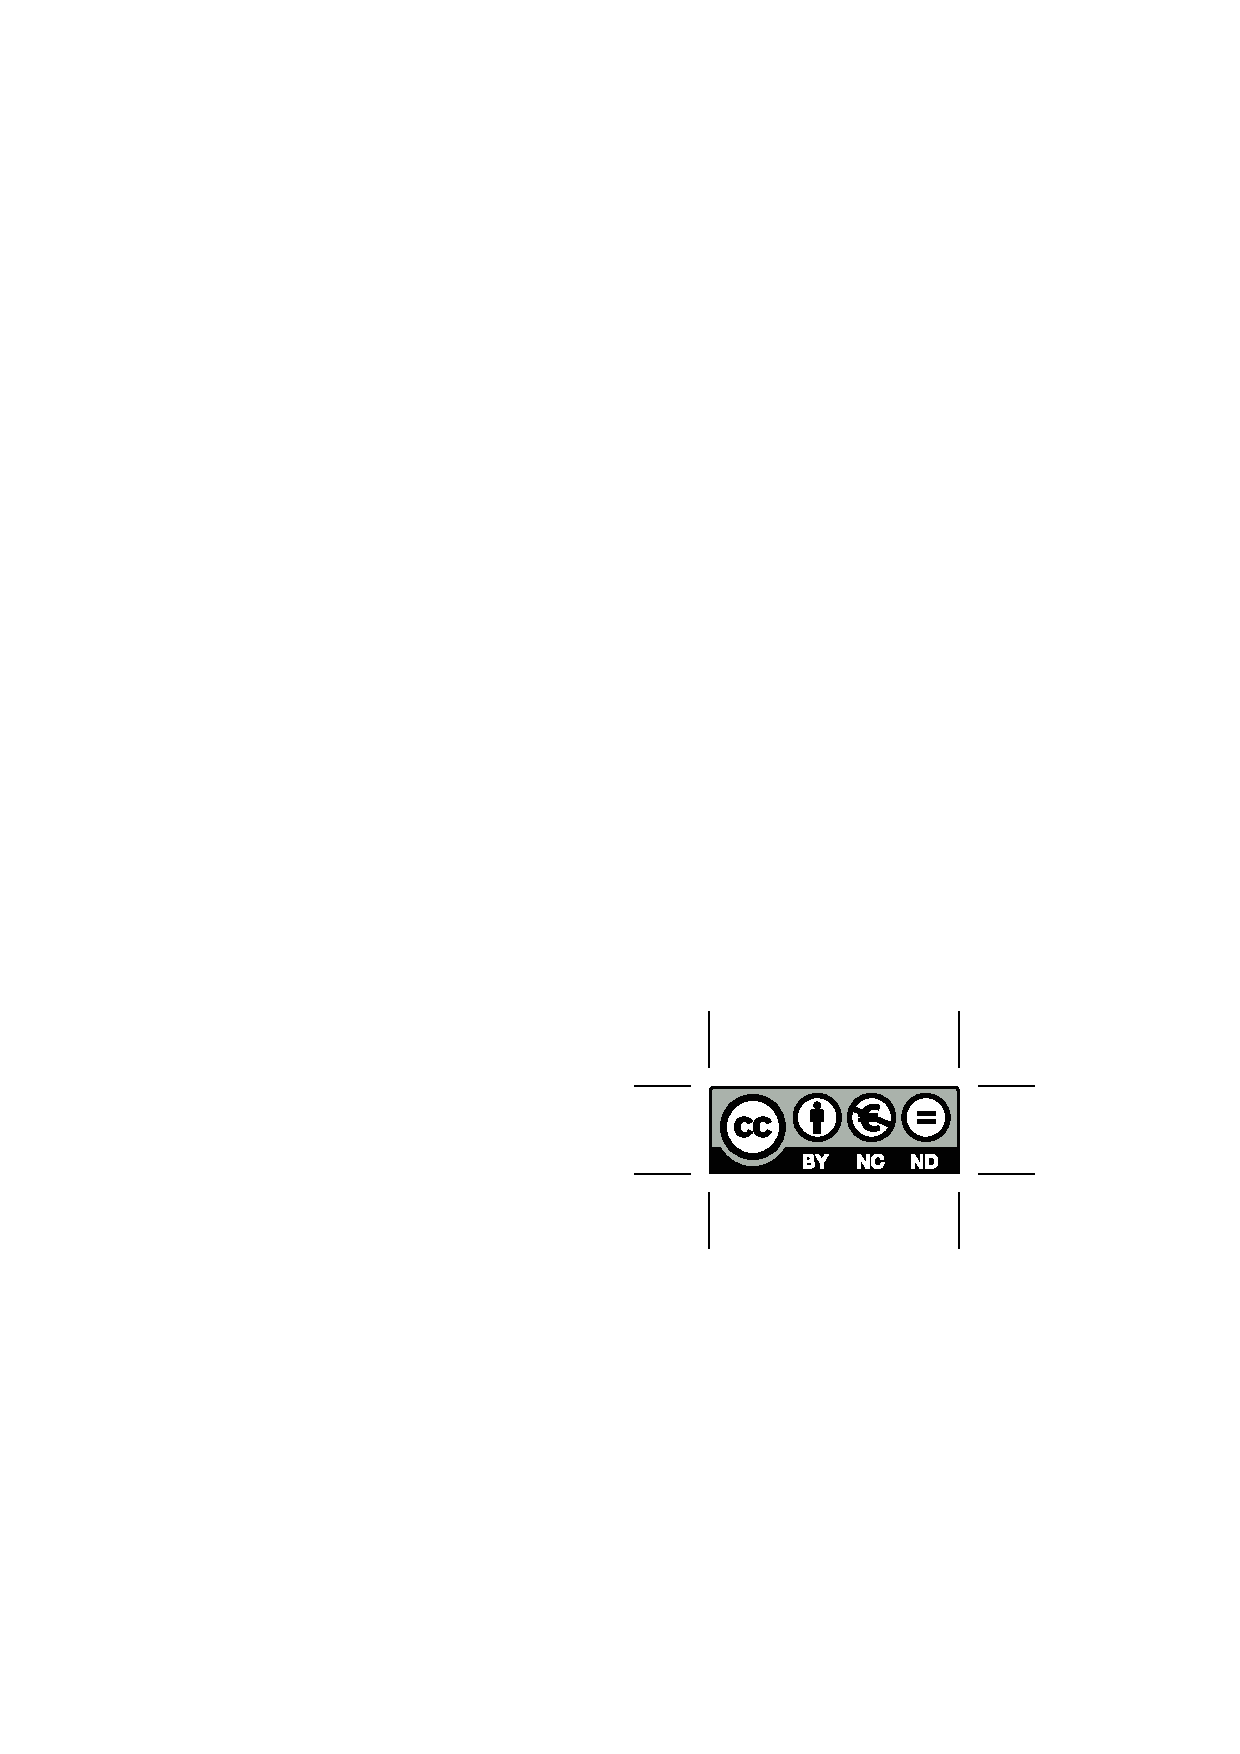
\includegraphics[height=35px]{by-nc-nd-eu}
        \end{minipage}\hfill
    \end{center}

    Cette \oe{}uvre est mise à disposition selon les termes de la \href{https://creativecommons.org/licenses/by-nc-nd/4.0/deed.fr}{Licence Creative Commons Attribution - Pas d’Utilisation Commerciale - Pas de Modification 4.0 International}. % consultez les conditions de la licence cc by-nc-nd, vous pouvez appliquer une licence moins restrictive, cc by-nc-sa par exemple
\fi

\iffalse % Affidavit of Honour for english thesis (invert the \if for an English thesis)
    I, undersigned, [First Name Surname], %% First Name and Surname of the PhD student
    hereby declare that the work presented in this manuscript is my own work, carried out under the scientific supervision of [First Name Surname], %% First Name and Surname of the thesis director and if applicable of the co-thesis director
    in accordance with the principles of honesty, integrity and responsibility inherent to the research mission. The research work and the writing of this manuscript have been carried out in compliance with both the french national charter for Research Integrity and the Aix-Marseille University charter on the fight against plagiarism.
    
    This work has not been submitted previously either in this country or in another country in the same or in a similar version to any other examination body.\\
    
    [Place] [date]
    
    \begin{flushright}\includegraphics[width=120px,height=40px]{example-image-a}\end{flushright}% signature

    ~\vfill
    \begin{center}
        \begin{minipage}[c]{0.25\linewidth}
            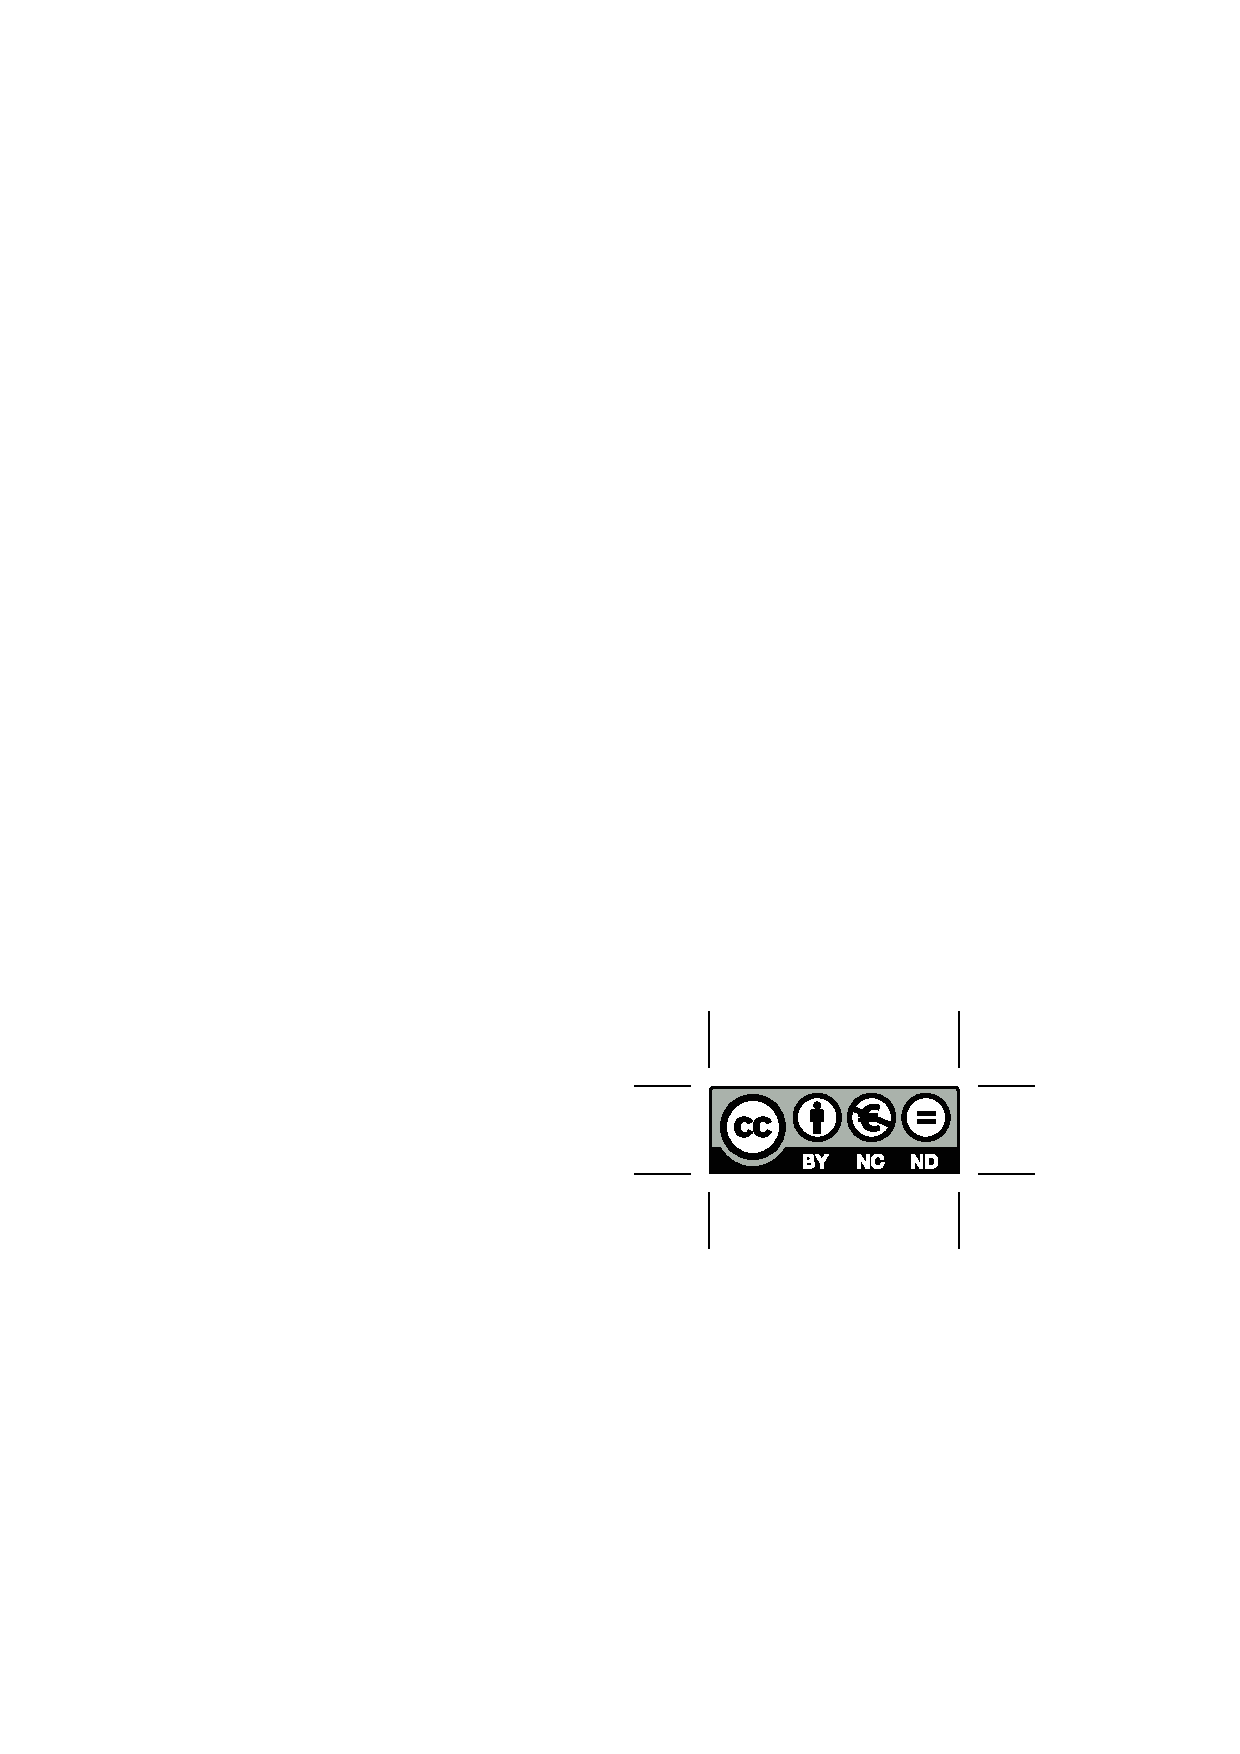
\includegraphics[height=35px]{by-nc-nd-eu}
        \end{minipage}\hfill
    \end{center}

    This work is licensed under \href{https://creativecommons.org/licenses/by-nc-nd/4.0/deed.en}{Creative Commons Attribution-NonCommercial-NoDerivatives 4.0 International Public License}
\fi

				%% affidavit et licence

	\newpage
\addchap{Liste de publications et participation aux conférences}
\label{chap:publications}
\addsec*{Liste des publications et/ou brevets réalisées dans le cadre du projet de thèse:}
\begin{enumerate}
\item 
\item 
\item 
\end{enumerate}


\addsec*{Participation aux conférences et écoles d’été au cours de la période de thèse:}
\begin{enumerate}
\item 
\item 
\item 
\end{enumerate}			%% liste de publications et participation aux conférences

	\addchap{Résumé et mots clés}
\label{chap:resume}
\lipsum[1]\index{Lorem ipsum}

\vspace{0.5cm}
Mots clés: géométrie algorithmique, complexe planaire et rectangulaire, géodésique, courbure globale non-positive
					%% résumé

	\addchap{Abstract and keywords}
\label{chap:abstract}
\selectlanguage{english}
\lipsum[1]\index{Lorem ipsum}

\vspace{0.5cm}
Keywords: computational geometry, planar and rectangular complex, geodesic, global nonpositive curvature
\selectlanguage{french}
				%% abstract

	\addchap{Remerciements}
Le modèle de thèse AMU n'existerait pas sans la contribution des doctorants. Nous souhaitons remercier tout particulièrement \href{http://www.theses.fr/2011AIX20720}{Mickaël Bojados}, \href{http://www.theses.fr/2011AIX22111}{Flora Cordoleani} et \href{http://www.theses.fr/2014AIXM4013}{Florian Caullery} pour leur aide précieuse et la qualité de leurs fichiers sources LaTeX. La mise à jour effectuée en 2018 doit beaucoup à l'excellent travail de \href{http://theses.fr/2014ENMP0038}{Dorian Depriester}.

\lipsum[1-2]\index{Nam dui ligula}
				%% remerciements

    \microtypesetup{protrusion=false}	%% désactive la protrusion (TOC LOFT GLS)
	\tableofcontents					%% TOC
	\listoffigures						%% LOF
	\listoftables						%% LOT
	\printglossary[						%% acronymes
		type=\acronymtype,
		title={Liste des acronymes},
		toctitle={Liste des acronymes}
		]
	\printglossary[						%% glossaire
		title={Glossaire},
		toctitle={Glossaire}
		]
	\printglossary[						%% nomenclature
		type=notation,
		title={Nomenclature},
		toctitle={Nomenclature}
		]
    \microtypesetup{protrusion=true}	%% rétabli la protrusion

	\ohead{\leftmark\Ifstr{\rightmark}{\leftmark}{}{ -- \rightmark}}	%% place le chapître et la partie en en-tête

	\addchap{Introduction}

The increasing global demand for energy, coupled with the urgent need to reduce greenhouse gas emissions, has driven the search for more efficient and sustainable energy solutions. 
Traditional energy generation methods, such as coal-fired power plants and natural gas turbines, contribute significantly to environmental pollution and are often limited by their 
thermodynamic efficiencies. In this context, supercritical fluids, particularly supercritical carbon dioxide (sCO2), have gained attention due to their unique properties and 
potential to revolutionize energy generation systems.
Supercritical CO2 is a state of carbon dioxide achieved when it is heated and pressurized above its critical point (31.1°C and 7.38 MPa). 
In this supercritical state, CO2 exhibits properties of both a liquid and a gas, resulting in a dense, compressible fluid with excellent thermal conductivity and diffusivity. 
These properties make sCO2 an ideal working fluid for various thermodynamic cycles, especially the Brayton cycle.




	\chapter{Fluid simulation}
\chaptertoc{}

In fluid simulation, there are different approaches: the microscopic, 
the mesoscopic, and the macroscopic approach. In the microscopic approach, 
all the interactions between molecules are modeled. While this method provides a 
highly detailed representation of the fluid's behavior, it is extremely 
time-consuming due to the complexity of calculating every molecular interaction.

The mesoscopic approach, on the other hand, is based on kinetic theory. In this 
approach, a group of molecules is treated as a single entity. This method relies 
on statistical mechanics to describe the distribution of particles in a fluid and
how this distribution evolves over time. It provides a balance between 
computational efficiency and accuracy by focusing on the collective behavior of 
particles rather than individual interactions.

The macroscopic approach is the classical method, where the fluid is treated by
considering only its macroscopic properties, such as velocity, pressure, and 
temperature. This method typically involves solving the Navier-Stokes (NS) 
equations, which describe the motion of fluid substances.

In this manuscript, the mesoscopic approach is utilized, specifically through
 the Lattice Boltzmann Method (LBM). The LBM has proven its efficiency in 
 simulating fluid dynamics by significantly improving computational speed compared 
 to classical NS solvers.

To achieve this, some fundamental concepts from kinetic theory are introduced,
followed by an overview of the classical Lattice Boltzmann Method. 
Subsequently, the method used for the simulation of supercritical 
CO\textsubscript{2} is presented.

\section{Fundamentals on kinetic theory}

\section{Fundamentals on Lattice Boltzmann Method}

The Lattice Boltzmann Method (LBM) was developed in the late 1980s and has been used
for Computational Fluid Dynamics (CFD) since then. Specifically, the foundational
work on LBM can be traced back to the work of Frisch, Hasslacher, and Pomeau in 
1986, who introduced the Lattice Gas Automaton (LGA), which is the precursor to 
LBM. The LBM, as it is known today, evolved from these early developments in the 
late 1980s and early 1990s. This first method was only used for weakly compressible
flows, where the temperature is constant and a perfect gas equation is used to close
the system and being equivalent to a Navier-Stokes formulation. The method has 
evelouated from that basic formulation and nowadays permits the use of difficult 
equations of state and the use for High compressible flows. 
This section provides the main concepts and expressions used in the classical and 
more simplest LBM. For doing that, a brief introduction of the Boltzmann equation
is made. 

\subsection{Boltzmann equation}
The Boltzmann equation, formulated by Ludwig Boltzmann in 1872, is a fundamental
equation in statistical mechanics that describes the statistical behavior of a 
thermodynamic system out of equilibrium. It is used to study the dynamics of a 
gas at the microscopic level by considering the distribution function 
f($x$,$\xi$,$t$), which represents the number of particles at a given 
position $x$, with a given velocity $\xi$, at time $t$.

In order to see the time evolution, the total derivative of the distribution
function can be expressed as:

\begin{equation}
	\frac{\mathrm{d}f}{\mathrm{d}t} = 
	\left(\frac{\partial f}{\partial t}\right)\frac{\mathrm{d}t}{\mathrm{d}t}
	+\left(\frac{\partial f}{\partial x_{\beta}}\right)\frac{\mathrm{d}x_{\beta}}{\mathrm{d}t}
	+\left(\frac{\partial f}{\partial \xi_{\beta}}\right)\frac{\mathrm{d}\xi_{\beta}}{\mathrm{d}t}
\end{equation}

Looking each term, we can indentify and define $\frac{\mathrm{d}f}{\mathrm{d}t} = \Omega(f)$
as the collision operator, $\frac{\mathrm{d}t}{\mathrm{d}t}=1$, 
the particle velocity as $\frac{\mathrm{d}x_{\beta}}{\mathrm{d}t} = \xi_{\beta}$
and $\frac{\mathrm{d}\xi_{\beta}}{\mathrm{d}t} = \frac{F_{\beta}}{\rho}$.

Leading to the final expresion for the Boltzmann equation.

\begin{equation}
	\Omega(f) = \frac{\partial f}{\partial t} 
	+ \xi_{\beta}\frac{\partial f}{\partial x_{\beta}}
	+ \frac{F_{\beta}}{\rho}\frac{\partial f}{\partial \xi_{\beta}}
\end{equation}

This expression can be seen as an advection equation for the distribution 
function, where the collision operator acts as a source term.

In the first equation developed by Ludwig Boltzmann, the formulation for
the collision operator involved complex integrals and cumbersome mathematical 
operations, making the calculations difficult to achieve. In 1954, 
P. L. Bhatnagar, E. P. Gross, and M. Krook introduced the BGK collision 
operator in their seminal paper titled "A Model for Collision Processes 
in Gases. I. Small Amplitude Processes in Charged and Neutral One-Component 
Systems," published in Physical Review. The BGK collision operator 
simplifies these calculations by incorporating only a single relaxation time.

The next subsection is dedicated to show a little bit about the BGK collision 
operator and how it was constructed.

\subsection{BGK collision operator}

\section{Unified Lattice Boltzmann method}

	\chapter{ Thermodynamics}
\chaptertoc{}

\section{Ideal Gas EoS}

A mathematical relationship that connects temperature, pressure, and volume is
known as an Equation of State (EOS). These equations can be expressed in either
a pressure-explicit form (such as CEOS) or a volume-explicit form. The ideal gas
(IG) model is the most basic theoretical representation of a gas, grounded in
the principles of kinetic theory. This model is based on the key assumption that
the gas consists of point-like particles, which interact only through elastic
collisions, with no long-range intermolecular forces. The main advantage of this
simplified model is its straightforward and easy-to-use EOS, which is described
below:

\begin{equation}
	P = \frac{RT}{V}
\end{equation}

Where $P$ represents the gas pressure, $V$ is the molar volume, $T$ is the
temperature, and $R$ is the ideal gas constant. This equation can also be
expressed in a specific form as follows:

\begin{equation}
	P = \frac{rT}{v} = \rho rT
\end{equation}

Where $\rho = \frac{1}{v}=\frac{M}{V}$ represents the density, $M$ is the fluid's molecular weight, , $v$ is the specific volume of the fluid, and $r$ is known as the specific gas constant:

\begin{equation}
	r = \frac{R}{M}
\end{equation}

	\subsection{Heat capacities, enthalpy and entropy}

	Using the Ideal Gas Equation of State (IG EOS), the following standard
	relationships apply:
	
	\begin{enumerate}
		\item Mayer's relation:
		\begin{equation}
			C_P - C_V = R
		\end{equation}

		\item Variation in internal energy:
		\begin{equation}
			\mathrm{d}E = C_V\mathrm{d}T
		\end{equation}

		\item Variation in enthalpy:
		\begin{equation}
			\mathrm{d}H = C_P\mathrm{d}T
		\end{equation}

		\item Variation in entropy:
		\begin{equation}
			\mathrm{d}S = \frac{C_P}{T}\mathrm{d}T - R\frac{\mathrm{d}P}{P}
		\end{equation}

	\end{enumerate}

	\subsection{NASA Polynomials}
	
	In its simplest form, the Ideal Gas Equation of State (IG EOS) assumes
	constant heat capacities, leading to linear relationships between enthalpy
	and internal energy with respect to temperature. However, this assumption is
	not valid across a wide range of temperatures. For example, in the field of
	combustion, the NASA polynomial model is commonly used to describe heat
	capacities more accurately. The NASA-7 model, for instance, expresses heat
	capacities in the following form [10]:

	\begin{equation}
		\frac{C_p}{R} = a_1 + a_2 + a_3 T^2 + a_4 T^3 + a_5 T^4
	\end{equation}

	\begin{equation}
		\frac{H}{RT} = a_1 + \frac{a_2}{2}T + \frac{a_3}{3}T^2 + \frac{a_4}{4}T^3 + \frac{a_5}{5}T^4 + \frac{a_6}{T}
	\end{equation}

	\begin{equation}
		\frac{S}{R} = a_1 \ln T + a_2 T + \frac{a_3}{2}T^2 + \frac{a_4}{3}T^3 + \frac{a_5}{4}T^4 + a_7
	\end{equation}
	The ideal gas equation of state (EOS) is a straightforward yet accurate
	model for describing gas behavior at high temperatures and relatively low
	pressures. However, it falls short in representing condensed fluids. Despite
	this limitation, the ideal gas model has been extensively studied and
	documented over the years. Consequently, many thermodynamic problems
	transition from the Real Gas (RG) state to the Ideal Gas (IG) state using
	residual or departure functions (see Section 2.4.3.2) to leverage the wealth
	of existing knowledge associated with the IG model.


	\subsection{Compressibility Factor}

	Real fluids at low density and high temperature can be accurately modeled by
	the perfect gas equation of state (EOS). However, at lower temperatures or
	higher densities, a real fluid deviates significantly from ideal gas
	behavior, especially during phase changes, such as when it condenses from a
	gas to a liquid or deposits from a gas to a solid. This deviation is
	quantified by the compressibility factor, $Z$, which indicates how much the
	fluid's behavior differs from that of an ideal gas:

	\begin{equation}
		Z = \frac{PV}{RT} =\frac{Pv}{rT} = \frac{P}{\rho RT} 
	\end{equation}

\section{Supercritical Fluids}

Supercritical phenomena are crucial in various industrial applications,
particularly in power cycles and energy recovery, which are the focus of this
work. This section is dedicated to understanding the key differences between
supercritical and subcritical fluids, with an emphasis on their role in power
generation.

Supercritical fluids, especially supercritical carbon dioxide ($CO_2$) and water,
are increasingly important in the development of advanced power cycles due to
their exceptional thermodynamic properties. These fluids are used to enhance
efficiency, reduce the size of equipment, and minimize environmental impact in
power generation systems. Here are some key applications:

    Supercritical $CO_2$ Power Cycles: Brayton Cycle: Supercritical $CO_2$ is a
        promising working fluid in closed-loop Brayton cycles, where it operates
        at temperatures and pressures above its critical point. These cycles
        have the potential to surpass the efficiency of traditional steam
        Rankine cycles, primarily because supercritical $CO_2$ has a higher
        density, which allows for more compact and efficient turbomachinery.
        This increased efficiency translates into lower fuel consumption and
        reduced greenhouse gas emissions, making supercritical $CO_2$ Brayton
        cycles a leading candidate for next-generation power plants. Waste Heat
        Recovery: One of the significant advantages of supercritical $CO_2$ cycles
        is their ability to recover waste heat from industrial processes, gas
        turbines, and even nuclear reactors. By utilizing waste heat, these
        systems can generate additional electricity without burning extra fuel,
        improving the overall efficiency of energy systems and reducing the
        carbon footprint of power generation.

    Supercritical Water Power Cycles: Supercritical Water-Cooled Reactors
        (SCWRs): In nuclear power generation, supercritical water is used as a
        coolant in advanced reactor designs. SCWRs operate at supercritical
        pressures and temperatures, allowing for higher thermal efficiency
        compared to conventional reactors. This not only improves the power
        output but also contributes to the safety and economic viability of
        nuclear energy.

    Supercritical Steam Cycles: Traditional fossil fuel power plants are
        evolving with the adoption of supercritical and ultra-supercritical
        steam cycles. By operating at temperatures and pressures above the
        critical point of water, these power plants achieve higher thermal
        efficiencies, reducing fuel consumption and emissions. The move towards
        supercritical steam cycles represents a significant advancement in
        making coal-fired power generation cleaner and more efficient.
		
    Hybrid Power Cycles: Integration with Renewable Energy: Supercritical $CO_2$
        and water cycles are being integrated with renewable energy sources,
        such as concentrated solar power (CSP) and geothermal energy. In CSP
        plants, supercritical $CO_2$ is used to transfer heat from the solar field
        to the power block, allowing for more efficient energy conversion.
        Similarly, in geothermal systems, supercritical fluids can enhance
        energy extraction from deep, high-temperature reservoirs, providing a
        reliable and sustainable source of electricity. Combined Cycle Plants:
        In combined cycle power plants, supercritical $CO_2$ can be used in
        conjunction with gas turbines to further increase overall efficiency.
        The exhaust heat from the gas turbine is used to generate additional
        power in a supercritical $CO_2$ cycle, making these plants among the most
        efficient forms of fossil fuel-based power generation.

    Environmental Benefits and Future Potential: Carbon Capture and Utilization:
        Supercritical $CO_2$ power cycles not only improve efficiency but also
        facilitate carbon capture and utilization (CCU). By integrating CCU with
        supercritical $CO_2$ cycles, power plants can reduce their carbon emissions
        while potentially producing valuable products like synthetic fuels. This
        dual benefit supports the transition to more sustainable energy systems.
        Future Research and Development: Ongoing research into supercritical
        fluid power cycles is focused on optimizing system design, improving
        materials that can withstand the harsh conditions of supercritical
        operation, and integrating these cycles with emerging technologies. The
        goal is to create highly efficient, low-emission power plants that can
        meet the growing global demand for electricity while minimizing
        environmental impact.

In conclusion, supercritical fluids are at the forefront of power generation
technology, offering significant advantages in efficiency, compactness, and
environmental sustainability. As research and development continue, these
systems are expected to play a central role in the future of energy, making them
a critical area of study for advancing power cycles and reducing the carbon
footprint of electricity generation.

In order to star with a better comprehension of the supercritical state
comprehension, some reduced parameters are introduced:

\begin{equation}
	Pr = \frac{P}{P_c}
\end{equation}

\begin{equation}
	T_r = \frac{T}{T_c}
\end{equation}

\begin{equation}
	V_r = \frac{V}{V_c}
\end{equation}

\begin{equation}
	\rho_r = \frac{\rho}{\rho_c}
\end{equation}

where subscript $c$ denotes the parameter's value at the critical point.

	\subsection{Physical Structure of Supercritical Fluids}

	The first topic to address is the nature of supercritical fluids. It is
	well-known that, in the supercritical state, there is no distinctly separate
	phase (see Figure 2.1) [14].

	Using molecular dynamics simulations of liquid and transcritical states at a
	reduced temperature of 0.5 and reduced pressures of 0.7, 1.4, and 3.0,
	Banuti [15] demonstrated that there is no need to separate quadrants IL and
	IV in Figure 2.1. This is because densely packed fluids in IL exhibit the
	same physical behavior as their supercritical counterparts in IV. For gases,
	however, the equivalency between the supercritical fluid and the ideal gas
	model in the ($P_r,T_r$) plane is reduced to a line. It is important to
	note that, up to $P_r=3$ and for $T_r>2$, describing a supercritical
	fluid as an ideal gas results in a compressibility factor error of less than
	5$\%$, as shown in Figure 2.2.

	Consequently, a pseudo-transition should exist, dividing the supercritical
	region, as illustrated in Figure 2.1. Recent independent studies by Gorelli
	et al. [17] and Simeoni et al. [18], using X-ray scattering, have shown that
	sound dispersion, typically observed only in liquids, indeed occurs in a
	supercritical transition. This suggests that there are two distinct
	pseudo-states within supercritical matter, implying the existence of a
	mechanism analogous to a subcritical phase transition.

	\subsection{Pseudo-Boiling} % entre [] pour le texte dans la TOC
		\subsubsection{The Widom line}
		The existence of this pseudo-transition is confirmed at loci where the
		isobaric heat capacity ($C_p$) exhibits a relative maximum, either at
		constant pressure or constant temperature, in the ($P_r,T_r$) plane.
		These two definitions correspond to the Widom Line and the Characteristic
		Isobaric Inflection Curve (CIIC), respectively. Recently, Lamorgese et al.
		compiled classical cubic Equation of State (EOS) results to map the Widom
		Line locus [19].

		Banuti, however, advanced this understanding further. By applying the
		theoretical definition of an equilibrium state—where Gibbs free energy is
		equal—and using a correlation from Waring [20] along with a
		Soave-Redlich-Kwong-based calculation of the subcritical coexistence line's
		slope, he proposed a similarity law that aligns both the coexistence and
		Widom lines across a range of fluids [21]. The strength of Banuti's approach
		lies in its solid theoretical foundation, its adaptability to various
		fluids, and its simplicity.

		\begin{equation}
			P_r = exp\left[\frac{A_s}{min(T_r,1)}(T_r-1)\right]
		\end{equation}

		where $A_s$ is the critical slope of the coexistence line and can be
		calculated using a cubic Equation of State. For example, applying
		the Soave-Redlich-Kwong EOS results in the following expression:

		\begin{equation}
			A_{SRK} = 5.51934 + 4.80640\omega - 0.537437\omega^2
		\end{equation}
		
		where $\omega$ is the acentric factor of the considered species [21]. The
		corresponding scaling parameter is defined as:

		\begin{equation}
			P_r^* = P_r^{\frac{A_0}{A_s}}
		\end{equation}

		where $A_0$ is the result of Eq. (2.19) for a zero acentric factor. This
		scaling parameter is illustrated graphically in Figure 2.3 below.

	\subsection{Supercritical Latent Heat}

	To highlight the differences between subcritical and supercritical phase
	transitions, Banuti [22] illustrated the contrast between low-pressure and
	high-pressure state transitions. As shown in Figure 2.4, at low pressures,
	the latent heat $\Delta h_{th}$ required to overcome intermolecular forces is
	gradually replaced by a thermal shielding effect $\Delta h_{th}$ at higher
	pressures. This effect forces the fluid to heat up before it can undergo the
	transition.

	Furthermore, the pseudo-boiling phenomenon involves both dynamic and
	thermodynamic state transitions [23]. Banuti et al. note in their study that
	at very high pressures, this transition loses its thermodynamic nature and
	is replaced by a dynamic shift from rigid to non-rigid liquids, which no
	longer display liquid-like dispersion behavior.

	Section 2.3 highlights the need for an accurate thermodynamic description of
	heat capacities. Models of transport properties, such as thermal conductivity,
	are discussed in Chapter 3 to ensure a proper understanding of supercritical
	(SC) behavior.

			
\section{Cubic EoS}

In this section, some of the most popular cubic equations of state (CEOS) are
introduced. Energy changes are expressed by applying the results from the
previous section. The widespread use of these equations is due to three key
reasons [4, 24]:

    They are applicable across a wide range of pressures and temperatures. They
    can represent compounds in both liquid and vapor phases. They are
    well-suited for the study of supercritical fluids.

All thermodynamic properties presented in this chapter are either obtained from
the NIST Chemistry WebBook [16] or calculated using some EOS.
		
	\subsection{A bit of history}
	This first section provides a brief historical overview of the EOS class
	under consideration.

	\subsubsection{The Corresponding States Principle and Criticalicity Condition}
	Van der Waals introduced the Corresponding States Principle (CSP) with the
	statement: 'Substances behave alike at the same reduced states. Substances
	at the same reduced states are in corresponding states.' This principle is
	of fundamental importance when considering supercritical fluids, as it
	introduces the critical point of a fluid (denoted by the subscript $\phi_c$) as
	a scaling factor, allowing for comparisons between different compounds. The
	concept gave rise to the widely used 'reduced' thermodynamic variables. The
	critical point serves as the ideal scaling reference for the application of
	the corresponding states principle due to the existence of specific
	criticality conditions, which are as follows:

	\begin{equation}
		\left(\frac{\partial P}{\partial V}\right)_{T=T_c}
	\end{equation}

	\begin{equation}
		\left(\frac{\partial^2 P}{\partial V^2}\right)_{T=T_c}
	\end{equation}

	These conditions express the fact that the saturation curve reaches a
	maximum at the critical point, and that the critical isotherm exhibits an
	inflection point at this same critical point. In fact, the attractive and
	repulsive parameters in cubic equations of state (CEOS) are derived from
	these critical conditions, making all compounds comparable under the
	Corresponding States Principle (CSP)

	\subsubsection{Van der Waals EOS}
	Historically, cubic equations of state (EOS) have been expressed in
	pressure-explicit form. They were specifically designed to account for
	intermolecular forces and accurately depict multiphase behavior. Van der
	Waals was the first to address this challenge, introducing the first cubic
	EOS, for which he was awarded the Nobel Prize in 1910 [25]. His
	straightforward formulation utilizes two constant parameters, aa and bb, to
	model attractive and repulsive forces, respectively

	\begin{equation}
		P = \frac{RT}{V-b} - \frac{a}{V^2}
	\end{equation}

	This formulation was developed into various equations of state (EOS)
	throughout the second half of the 20th century, particularly to refine the
	attractive term and make it more complex and accurate for different
	applications.

	\subsubsection{Redlich and Kwong's modification}
	
	In 1949, Redlich and Kwong, building on Van der Waals’ hard-sphere term,
	introduced an improved equation of state (EOS) by incorporating a more
	detailed temperature dependency into the attractive term [27]. This
	modification allowed their EOS to provide more accurate predictions of fluid
	behavior, particularly for gases near the critical point:

	\begin{equation}
		P = \frac{RT}{V-b} - \frac{a}{\sqrt(T_r)}\frac{1}{V(V+b)}
	\end{equation}

	Its widespread success stemmed from its adaptability, as Chueh and Prausnitz
	demonstrated that it could accurately predict both liquid and vapor
	saturation properties [28, 29].

	\subsubsection{Acentric factor introdction}

	Despite their success, both of these cubic EOS models fall short in
	representing the geometric complexity and polar properties of certain
	molecules. As illustrated in Figure 2.5, in complex polar
	compounds,intermolecular forces arise from locations other than the
	molecular centers.

	To address this issue, Pitzer introduced the acentric factor $\omega$ in 1955
	[30], as a measure of how much the thermodynamic properties of a substance
	deviate from those predicted by the Corresponding States Principle (CSP).

	\subsubsection{Soave's contribution}

	In 1972, Soave, recognizing the significance of Pitzer's acentric factor,
	extended the Redlich-Kwong equation of state (EOS) to create the widely
	known Soave-Redlich-Kwong (SRK) EOS [31]:

	\begin{equation}
		P = \frac{RT}{V-b}-\frac{a[1+K_{SRK}(\omega)(1-\sqrt(T_r))]^2}{V(V+b)}
	\end{equation}

	\begin{equation}
		K_{SRK}(\omega) = 0.480 + 1.574\omega -0.176\omega^2
	\end{equation}

	This formulation is particularly well-suited for accurately predicting vapor
	pressure data and behavior in the near-critical region [24].

	\subsubsection{Peng-Robinson equation of state}

	In 1976, Peng and Robinson (PR) recognized that the SRK EOS overestimated
	the critical compressibility factor of fluids ($Z_{c,SRK} = 1/3$). In response,
	they proposed an alternative form for the attractive term along with a more
	complex volume dependency [32]:

	\begin{equation}
		P = \frac{RT}{V-b}-\frac{a[1+K_{SRK}(\omega)(1-\sqrt(T_r))]^2}{V^2 +2V -b^2}
	\end{equation}

	\begin{equation}
		K_{SRK}(\omega) = 0.37464 + 1.54226\omega -0.26992\omega^2
	\end{equation}

	This formulation improved the accuracy of liquid volume predictions and
	provided more precise results around the critical point ($Z_{c,PR} = 0.307$).

	\subsection{Derived Properties for a Generic CEOS}
	This section focuses on establishing thermodynamic properties derived from
	Cubic Equations of State (CEOS). To provide a foundation for this, we begin
	with a few key reminders. Basic relationships between energy functions are
	introduced, followed by the application of the first law of thermodynamics
	to present fundamental equations that link differential expressions of
	various thermodynamic variables. Maxwell's relations are also recalled.

	Next, we demonstrate that Helmholtz free energy can serve as a generating
	function for other thermodynamic quantities. The concept of residual properties
	is then introduced, and these are applied to CEOS to determine the final
	expressions for important state functions, based on a generic CEOS.

	\subsubsection{Few reminders}

	Basic Definitions: In this section, we revisit the definitions of key
	thermodynamic quantities, including specific enthalpy $h$, Helmholtz free
	energy $A_W$, Gibbs free energy $g$, and the compressibility factor $Z$.

	\begin{equation}
		h = e + P/\rho
	\end{equation}

	\begin{equation}
		A_W = e + Ts
	\end{equation}

	\begin{equation}
		g = h - Ts
	\end{equation}

	\begin{equation}
		Z = \frac{P}{\rho RT}
	\end{equation}


	\chapter{ Immersed Boundary Methods}

\section{Overview of the Immersed Boundary Method in CFD}
The Immersed Boundary (IB) Method is a computational approach in CFD used to
simulate fluid-structure interactions and complex boundary problems. It offers
flexibility in handling interfaces between fluids and solid structures, which
are represented within a fixed (usually Cartesian) grid, rather than requiring
body-fitted grids that conform to complex geometries. The IB method was
pioneered to study biological flows and has since expanded to a wide range of
fields including engineering, medicine, and environmental sciences. Below, we
trace the key developments that have shaped the evolution and application of the
IB method.

\subsection{Origins and Early Development: Peskin’s Work (1970s)}
The IB method was first introduced by Charles Peskin in the early 1970s to model
blood flow through heart valves. Peskin's approach was innovative in that it
allowed for the simulation of moving boundaries (such as the flexible heart
valves) within a fixed grid. Traditionally, simulating complex structures would
require deforming the mesh to match the structure, which is computationally
intensive and can lead to numerical instability.

Peskin's original IB method employed a two-phase approach:

\begin{enumerate}
    \item A Lagrangian representation for the boundary or interface, where
    discrete points represented the boundary, allowing for the flexibility of
    movement.
    \item An Eulerian grid for the fluid domain, which remained fixed in space.
\end{enumerate}

The Lagrangian points interact with the Eulerian grid through a smoothing
function, which distributes forces from the boundary to the fluid domain and
interpolates fluid velocities back to the boundary points.

\section{General Formulation}
Para ilustrar de manera grafica, la siguiente figura, muestra un esquema de como
se representan la parte fluida y solida en el metodo de fronteras sumergidas de
manera discreta.

En este esquema, se designa la parte fluida $\omega_f$ como nodos eulerianos
representados en color negro, mientras que la parte solida $\omega_s$ es
designada como Lagrangiana y en color rojo.  

Otra convecion que utilizada en la presente documento es la de utilizar letras
mayusculas para la parte Lagrangiana y minusculas para la parte euleriana.

En general, el metodo IB consiste en la representacion del solido por medio de
terminos fuente, ya sea de cantidad de movimiento o de energia. Es decir, en
lugar de representar completamente el solido, solo se veran sus efectos en los
puntos Lagrangianos. Estos efectos, luego seran repartidos hacia el campo
euleriano mediante una operacion conocida como Spreading.

\subsection{Source term in momentum equation}

This method originally was developed using the Navier Stokes equations. As a
first approach and to have a good comprehension of the method, a brief
demonstration using the classical Navier Stokes equations is showed. Then, a
similar development is developed but using the Lattice Boltzmann Method. After
making that, we can profite an reduce the algorithme using some properties and
characteristiques of the LBM.

\subsubsection{Similar to Navier Stokes developments}

La ecuacion general de la conservacion de la cantidad de movimiento en un fluido puede ser
descrita de la siguiente manera;

\begin{equation}
	\frac{\partial \rho u_\alpha}{\partial t} + \frac{ \partial(\rho u_\alpha u_\beta + p\delta_{\alpha\beta}-\Pi_{\alpha\beta})}{\partial x_\beta} = F
\end{equation}

\begin{equation}
	\frac{\partial \rho u_\alpha}{\partial t}  = F + RHS
\end{equation}

De esta ecuacion, podemos decir que el termino de fuerza representa la influencia del solido,
en el dominio fluido. Sin embargo por el momento este termino es desconocido.

Para obtener la funcion matematica que permite calcular el termino de fuerza, el
metodo se divide en dos etapas. Una primera etapa donde se realiza una
simualcion sin tomar en cuenta el termino fuerza, esta etapa es conocida como la
etapa de prediccion.

\begin{equation}
	\frac{\partial \rho u_\alpha}{\partial t}  = RHS
\end{equation}

Discretizando la ecuacion tenemos:
\begin{equation}
	\frac{ (\rho u)^* - (\rho u)^n}{\Delta t}  = RHS
\end{equation}

Si discretizamos la ecuacion original tenemos:
\begin{equation}
	\frac{ (\rho u)^{n+1} - (\rho u)^n}{\Delta t}  = RHS + F
\end{equation}

Si quisieramos que en un solo paso de tiempo, la velocidad alcance el valor de
la velocidad target, la expresion se transforma en: 

\begin{equation}
	\frac{ (\rho u)^{t} - (\rho u)^n}{\Delta t}  = RHS + F
\end{equation}

Finalmente tenemos que:

\begin{equation}
	F = \frac{(\rho u)^{t} - (\rho u)^*}{\Delta t}
\end{equation}


En resumen, para aplicar el metodo IB y poder determinar la influencia del
solido en el fluido, debemos aplicar dos veces la ecuacion de conservacion de
momento de mecanica de fluidos. Una primera vez para poder hacer una prediccion
y una segunda para poder hacer una correcion aplicando el termino de fuerza.





\section{Choice of interpolation kernel}
En la literatura existen diversos kernel de interpolacion, tales como los
propuestos por Peskin, Roma, etc. Estos Kernel deben de cumplir con ciertas
condiciones para poder permitir una buena interpoalcion y spreading para la
comunicacion entre el dominio fluido y el dominio solido. La principal
condicion es que el kernel sea de clase uno, $C_1$ al menos.

\begin{equation}
	\delta_h(x) = \frac{1}{h^3}\phi\left(\frac{x}{h}\right)\phi\left(\frac{y}{h}\right)\phi\left(\frac{z}{h}\right)
\end{equation}

En el presente trabajo de tesis se utiliso, el kernel dado por Peskin, el cual
tiene la forma siguiente:

\begin{equation}
	\phi(r) = \frac{1}{4}(1+cos(\frac{\pi r}{2}))
\end{equation}


\section{Weight calibration}
Como descrito anteriormente, la region solida definida de acuerdo al metodo de
fronteras sumergidas, tiene una dimension menos que la dimension del dominio
fluido. Esto provoca que no exista una reprocidad directa entre el campo
euleriano y lagrangiano, por ello, una calibracion es necesaria de realizar de
tal manera que existq una reciprocidad y conservacion entre ambos espacios.

\begin{equation}
	W_k = \frac{1}{\sum_l\sum_j\delta(x_j-X_K)\delta(x_j-X_l)}
\end{equation}

\section{Linking LBM with LBM}
In order to link this two methods, we have to use two steps, the prediction and
the corrector step.

\subsection{Prediction}
In the prediction step, all the calculations are made without the forces. Using
equation (\ref{explicit equivalent equation}) we have:

\begin{equation}
    \Bar{f}_i^* (t+\Delta t, x_i + c_i \Delta t) = \Bar{f}_i (t, x) + \Delta t \, \Omega_i (t, x_i)
\end{equation}

It seems that in this equation we eliminate the forces but in reality there
exist some force terms hidden in $\Bar{f_i}$.\footnote{Another important  thing
is to note that this equation is second order because it comes from the Cranck
Nicholson step, we can use an upwind scheme also but it's only first order} 

Using the definition of $\Bar{f_i}$, replacing in equation 8 and eliminating
also the hidden force terms: 

\begin{equation}
    f_i^* (t+\Delta t, x_i + c_i \Delta t) 
    - \frac{\Delta t}{2} \, \Omega_i (t+\Delta t, x_i + c_i \Delta t) 
    = f_i (t, x) 
    + \frac{\Delta t}{2} \, \Omega_i (t, x_i).
\end{equation}

\begin{equation}
    f_i^* (t+\Delta t, x_i + c_i \Delta t) 
    = f_i (t, x) 
    + \frac{\Delta t}{2} \left( \Omega_i (t, x_i) 
    + \frac{\Delta t}{2} \, \Omega_i (t+\Delta t, x_i + c_i \Delta t) \right).
\end{equation}

\begin{equation}
    f_i^* (t+\Delta t, x_i + c_i \Delta t) = f_i (t, x) + \frac{\Delta t}{2} \, (\text{RHS})
    \label{Prediction equation}
\end{equation}

\subsection{Correction}
In this part we are going to use the forcing term exactly as in equation
(\ref{explicit equivalent equation}).  

\begin{equation}
    \Bar{f_i^t}_{(t+\Delta t, x_i +c_i \Delta t)} = \Bar{f_i}_{(t,x)} + \Delta t(\Omega_i +F_i)_{(t, x_i)}
\end{equation}

Using the definition of $\Bar{f_i}$ we have:

\begin{equation}
    \Bar{f_i} (t+\Delta t, x_i + c_i \Delta t) = f_i (t, x) + \frac{\Delta t}{2} \left( \Omega_i + F_i \right)_{(t, x_i)}
\end{equation}  

\begin{equation}
    f_i^t (t+\Delta t, x_i + c_i \Delta t) 
    - \frac{\Delta t}{2} \left( \Omega_i + F_i \right)_{(t+\Delta t, x_i + c_i \Delta t)} 
    = f_i (t, x) 
    + \frac{\Delta t}{2} \left( \Omega_i + F_i \right)_{(t, x_i)}.
\end{equation}  

\begin{equation}
    f_i^t (t+\Delta t, x_i + c_i \Delta t) = f_i (t, x) 
    + \frac{\Delta t}{2} \left( \Omega_i + F_i \right)_{(t, x_i)} 
    + \frac{\Delta t}{2} \left( \Omega_i + F_i \right)_{(t+\Delta t, x_i + c_i \Delta t)}.
\end{equation}  

\begin{equation}
    f_i^t (t+\Delta t, x_i + c_i \Delta t) = f_i (t, x) 
    + \frac{\Delta t}{2} \left( \Omega_i (t, x_i) + \Omega_i (t+\Delta t, x_i + c_i \Delta t) \right) 
    + \frac{\Delta t}{2} \left( F_i (t, x_i) + F_i (t+\Delta t, x_i + c_i \Delta t) \right).
\end{equation}

\begin{equation}
    f_i^t (t+\Delta t, x_i + c_i \Delta t) = f_i (t, x) 
    + \frac{\Delta t}{2} (\text{RHS}) 
    + \frac{\Delta t}{2} \left( F_i (t, x_i) + F_i (t + \Delta t, x_i + c_i \Delta t) \right)
    \label{Correction equation}
\end{equation}

Subtracting equation (\ref{Prediction equation}) from (\ref{Correction
equation}):

\begin{equation}
    f_i^t (t+\Delta t, x_i + c_i \Delta t) - f_i^* (t+\Delta t, x_i + c_i \Delta t) 
    = \frac{\Delta t}{2} \left( F_i (t, x_i) + F_i (t + \Delta t, x_i + c_i \Delta t) \right)
    \label{IBM with LBM}
\end{equation}

Now applying the reconstruction to the equation (\ref{IBM with LBM}) in order to
have the macroscopic properties: 

\begin{equation}
    \rho u^t - \rho u^* = \frac{\Delta t}{2} (F_{(t)} + F_{(t+\Delta t)})
    \label{Real IBM LBM}
\end{equation}

We can see that if the force is constant the equations from Navier Stokes and
LBM are equal.

In a similar way, if we use a first order scheme for equation (8), we are going
to arrive to the Navier Stokes equation.

\section{An one step algorithme}
As seen before, all the demonstration was deducted solving to times the
Boltzmann equation. One time in order to determine the required force and a
second time using this force to find the good velocity, pressure, temperature,
etc field.

This is the classical way that was herited from the Navier Stokes developements,
but one advantage of using the Immersed Boundary method in the Lattice Boltzmann
framework is that in order to determine the force, we don't need to make a
prediction.

Using the defition of the variable change made in order to have a second order
algorithme, we can have an expression to apprximate the required force that
represents the effect of the solid on the fluid.

From the variable change, we have:

\begin{equation}
    \bar{f_i} = f_i - \frac{\Delta t}{2}({\Omega + F_i})
\end{equation}

Taking the first moment od the last equation we have:
\begin{equation}
    \sum{c_i\bar{f}} = \rho u_\alpha - \frac{\Delta t}{2}({\sum F_i})
\end{equation}

This equation is valid for all the times steps and positions. Suddenly if we
would like to compute the force term we need to known the value of the first
moment of the bar distribution function, but this value is unknown because we
need the force term to solve the Boltzmann method. This is why, in order to
approximate the force term, the previous value of the first moment is used. 

Finally, the expression to approximate the force term is:

\begin{equation}
    F_\alpha = 2(\rho u_\alpha - \sum {c_i\bar{f_i}})
\end{equation}

In this manuscript, the one step algorithme is used due the gain in time because
the LBM is going to be solved only one time.

\subsection{Energy source term}

The total energy equation is:

\begin{equation}
    \frac{\partial\rho E}{\partial t} + \frac{\partial\left[(\rho E +p)u_\beta + q_\beta - u_\alpha\Pi_{\alpha\beta}\right]}{\partial x_\beta} = \dot{Q}_{IBM}
\end{equation}

In a similar way that was made for the momentum equation, we can estimate the
IBM source term in order to represent the impact of a solid on the fluid. To
make that, a prediction of the temperature should be made. 

In this case the prediction of the temperture on the solid is going to be only
related with the temperature of the fluid around the solid using for that the
interpolation operator.

\begin{equation}
    \rho E^t - \rho E^{n} = \dot{Q}_{IBM}
\end{equation}

Where $E = e + \frac{1}{2}\rho u^2$, then:

\begin{equation}
    \rho {e^t + \frac{1}{2}\rho u^t}^2 - \rho {e^n - \frac{1}{2}\rho u^n}^{2} = \dot{Q}_{IBM}
\end{equation}

\begin{equation}
    \rho {e^t} - \rho {e^n} + {\frac{1}{2}\rho u^t}^2  - {\frac{1}{2}\rho u^n}^{2} = \dot{Q}_{IBM}
\end{equation}

\begin{equation}
    \rho {e^t} - \rho {e^n} + \left({\rho u^t}  - {\rho u^n}\right) \left(\frac{u^t + u^n}{2}\right) = \dot{Q}_{IBM}
\end{equation}

\begin{equation}
    \rho {e^t} - \rho {e^n} + \left(F_{IBM}\right) \left(\frac{u^t + u^n}{2}\right) = \dot{Q}_{IBM}
\end{equation}

What is interesting to see here is the presence of the force IBM. This term
represent the work of this force.

Another important remark in this model is that this source term for the energy
doesn't need a prediction step, we are going to use directly the interpolated
internal energy and the interpoleted velocity. This makes that the algorithme
should be solved only once. 

\section{Numerical implementation}
\section{Coupling with Lattice Boltzmann equations}
\subsection{Algorithme}
\begin{enumerate}
	\item Displacement of Lagrangian points according to the chosen physical
    model for boundary deformation; update of $U_d(X,t+\Delta t)$ and the
    interpolation and spreading operators based on the new geometry.

    \item Calculation of fi(x,t)
    
    \item Calculation of the IBM force 

    \item Solution of the discretized Boltzmann equation (2.9), yielding \(
    f_i(x, t + \Delta t) \) at the next time step.

    \item Calculation of the density \( \rho(x, t + \Delta t) \).

    \item Interpolation of the terms in equation (2.26) at time \( t + \Delta t
    \), and evaluation of the force \( F(X, t + \Delta t) \) on the Lagrangian
    points based on the desired velocity \( U_d(X, t + \Delta t) \).

    \item Spreading of the force \( F(X, t + \Delta t) \) onto the neighboring
    Eulerian points, yielding \( f(x, t + \Delta t) \) via equation (1.3).

    \item Update of the fluid state variables \( \rho(x, t + \Delta t) \) and \(
    u(x, t + \Delta t) \) at time \( t + \Delta t \) using equation (2.14),
    which includes the forcing term; return to step 1 for the next time step.
\end{enumerate}

	\addchap{Conclusion}
%\lipsum[1-2]


	\appendix

	\newpage
	\printbibliography[heading=bibintoc]%% bibliographie
	
	\newpage
	\printindex							%% index
	
	\newpage
	\printendnotes						%% notes

	%\setcounter{chapter}{0}
%\renewcommand{\thesection}{\Alph{section}}

\addpart{ANNEXES}

\chapter{Dynamic Pressure Equation}
\label{appendix:2ndOrderMoments}

The continuity equation serves as the starting point:

\begin{equation}
\frac{\partial \rho}{\partial t} + \frac{\partial (\rho u_\alpha)}{\partial x_\alpha} = 0.
\end{equation}

Multiplying the entire expression by the square of the lattice speed of sound \(c_s^2\) yields:

\begin{equation}
\frac{\partial (\rho c_s^2)}{\partial t} + c_s^2 \frac{\partial (\rho u_\alpha)}{\partial x_\alpha} = 0.
\end{equation}

To proceed, a low Mach number expansion of the density and velocity fields is performed:

\begin{equation}
\rho = \rho^{(0)} + M\!a^2 \rho^{(1)}, \qquad u_\alpha = u_\alpha^{(0)} + M\!a^2 u_\alpha^{(1)}.
\end{equation}

Substituting into the continuity equation yields:
\begin{align}
\frac{\partial\left( \rho^{(0)} + M\!a^2 \rho^{(1)} \right)c_s^2}{\partial t} 
+ c_s^2 \frac{\partial}{\partial x_\alpha}\left[ \left( \rho^{(0)} + M\!a^2 \rho^{(1)} \right)\left( u_\alpha^{(0)} + M\!a^2 u_\alpha^{(1)} \right) \right] = 0.
\end{align}

Expanding and collecting terms:
\begin{align}
\frac{\partial (\rho^{(0)})}{\partial t}  c_s^2
+ M\!a^2 \frac{\partial(\rho^{(1)})}{\partial t} c_s^2 
+ c_s^2 \frac{\partial}{\partial x_\alpha} \left( \rho^{(0)} u_\alpha^{(0)} 
+ M\!a^2 \left( \rho^{(1)} u_\alpha^{(0)} + \rho^{(0)} u_\alpha^{(1)} \right) \right) = 0.
\end{align}

The terms are now separated by Mach number order:

\paragraph{Zeroth-order (O(0)) terms:}
\begin{equation}
\frac{\partial(\rho^{(0)})}{\partial t} c_s^2 + c_s^2 \frac{\partial (\rho^{(0)} u_\alpha^{(0)})}{\partial x_\alpha} = 0,
\end{equation}
which is consistent with the continuity equation.

\paragraph{Second-order (O(M\!a\textsuperscript{2})) terms:}
\begin{equation}
\frac{\partial (\rho^{(1)} c_s^2)}{\partial t} + c_s^2 \frac{\partial}{\partial x_\alpha}(\rho^{(1)} u_\alpha^{(0)} + \rho^{(0)} u_\alpha^{(1)}) = 0.
\end{equation}

The dynamic pressure is defined as:

\begin{equation}
P_{\text{dyn}} = c_s^2 M\!a^2 \rho^{(1)},
\end{equation}

so the second-order equation becomes:
\begin{equation}
\frac{\partial P_{\text{dyn}}}{\partial t} + c_s^2 \frac{\partial}{\partial x_\alpha} \left( M\!a^2 (\rho^{(1)} u_\alpha^{(0)} + \rho^{(0)} u_\alpha^{(1)}) \right) = 0.
\end{equation}

To express this in terms of known variables, the mass flux is expanded:
\begin{align*}
\rho u_\alpha &= (\rho^{(0)} + M\!a^2 \rho^{(1)})(u_\alpha^{(0)} + M\!a^2 u_\alpha^{(1)}) \\
&= \rho^{(0)} u_\alpha^{(0)} + M\!a^2(\rho^{(0)} u_\alpha^{(1)} + \rho^{(1)} u_\alpha^{(0)}) + \mathcal{O}(M\!a^4).
\end{align*}

Neglecting higher-order terms, the second-order contribution is isolated:

\begin{equation}
M\!a^2 (\rho^{(1)} u_\alpha^{(0)} + \rho^{(0)} u_\alpha^{(1)}) = \rho u_\alpha - \rho^{(0)} u_\alpha^{(0)}.
\end{equation}

Substituting into the previous equation yields the final form:
\begin{equation}
\frac{\partial P_{\text{dyn}}}{\partial t} + c_s^2 \frac{\partial}{\partial x_\alpha} \left( \rho u_\alpha - \rho^{(0)} u_\alpha^{(0)} \right) = 0.
\end{equation}

This equation governs the evolution of the dynamic pressure and is valid under the low Mach number approximation.

\chapter{Consignes de présentation}
\label{chap:consignes}

Vous venez de télécharger la classe personnalisée LaTeX AMU pour les thèses de doctorat de l'université d'Aix-Marseille.
Certains éléments doivent obligatoirement être utilisés:
\\


\begin{figure}[h!tbp]
	%\vspace{0.5cm}
	\centering
	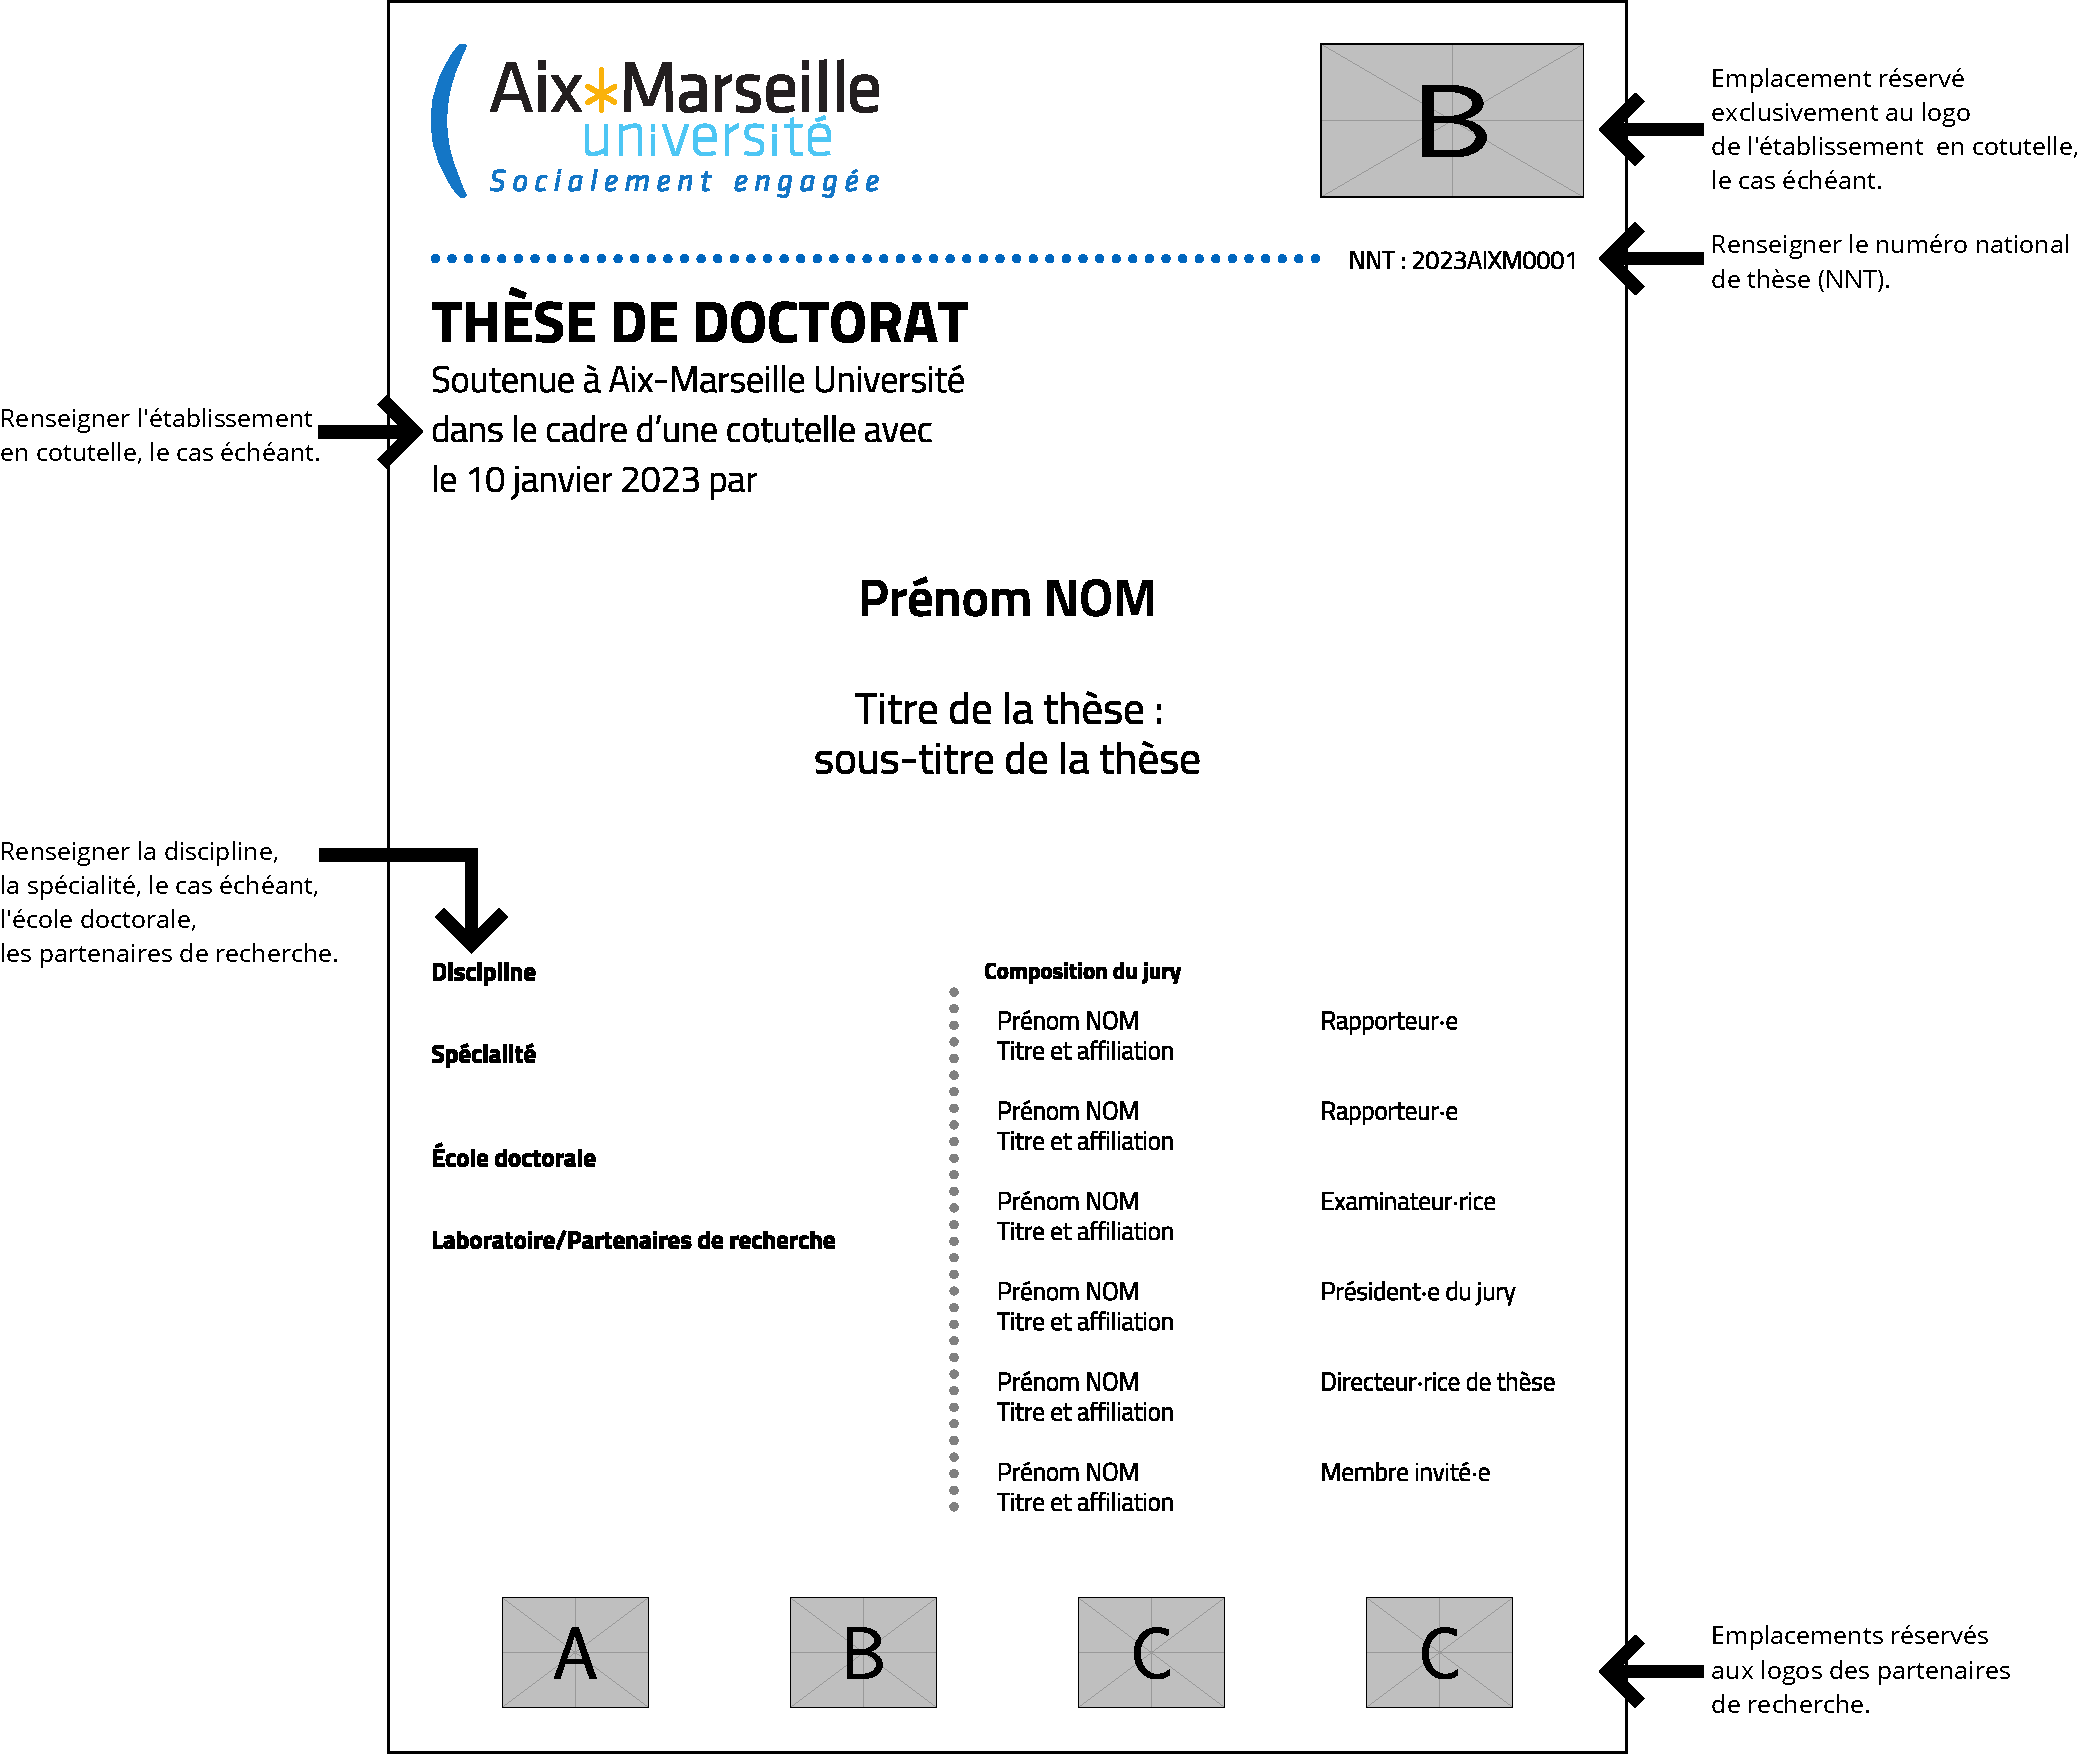
\includegraphics[width=0.8\textwidth]{titre.pdf}
\end{figure}

\begin{enumerate}
	\item La page de titre des thèses AMU: elle est rédigée en langue française avec la police Titillium, disponible avec le modèle LaTeX AMU aux formats TTF et TFM, selon la charte graphique AMU.
	\item En cas de cotutelle internationale, le logo de l’établissement partenaire doit apparaître en haut à droite de la page de titre;
	\item La composition du jury, l’école doctorale, la discipline et la spécialité (le cas échéant) doivent être conformes au formulaire ADUM de demande de soutenance de thèse;
	\item Le numéro national de thèse (NNT) doit être apposé sur la page de titre;
	\item Le cas échéant, les logos d’institutions ou d’unité de recherche partenaires peuvent être ajoutés en bas de la page de titre;
	\item La page \nameref{chap:affidavit}: selon la langue utilisée pour la rédaction de de votre thèse, opter pour la version en français ou en anglais, puis la compléter, la dater et la signer;
	\item La page \nameref{chap:publications} réalisées au cours de votre projet de thèse ;
	\item Les pages \nameref{chap:resume} en français et \nameref{chap:abstract} en anglais: chaque résumé ne doit pas dépasser 4000 caractères;
\end{enumerate}

Selon vos besoins, vous pouvez ajouter les éléments suivants: sommaire et/ou table des matières, liste des figures, liste des tableaux, liste des acronymes, glossaire, index, nomenclature…

Pour le corps de votre thèse, si votre école doctorale ne vous donne pas de consignes plus précises, vous pouvez utiliser les styles établis dans ce modèle ou vos propres styles en suivant ces recommandations:
\begin{itemize}
	\item Police neutre : Il est conseillé d'utiliser une police serif standard pour le texte et une police sans-serif standard pour les titres;
	\item Géométrie : paper=a4, fontsize=12pt, DIV=12;
	\item Interligne simple;
	\item Texte justifié.
\end{itemize}

\begin{figure}[h!tbp]
	%\vspace{0.5cm}
	\centering
	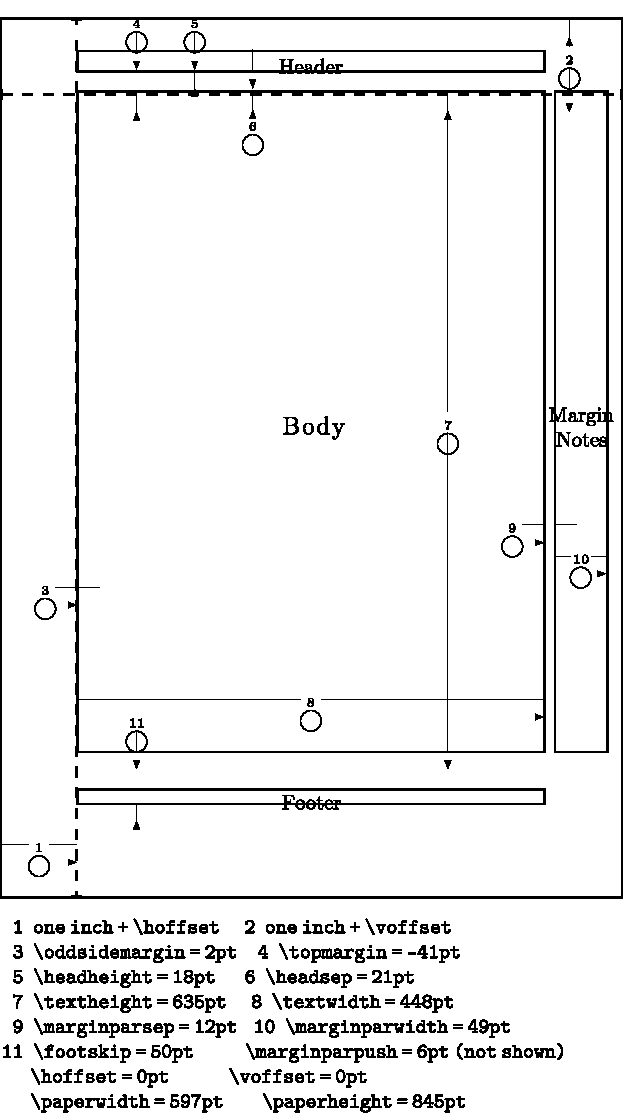
\includegraphics[width=0.3\textwidth]{geometry.pdf}
\end{figure}


Votre thèse devra être déposée en ligne en format PDF version 1.5 minimum sur \href{https://www.adum.fr/}{adum.fr}.



\chapter{Presentation guidelines}
\label{chap:guidelines}
\selectlanguage{english}
You have downloaded the LaTeX AMU custom class for Aix-Marseille University doctoral theses. Some elements must be used:
\\


\begin{figure}[h!tbp]
	%\vspace{0.5cm}
	\centering
	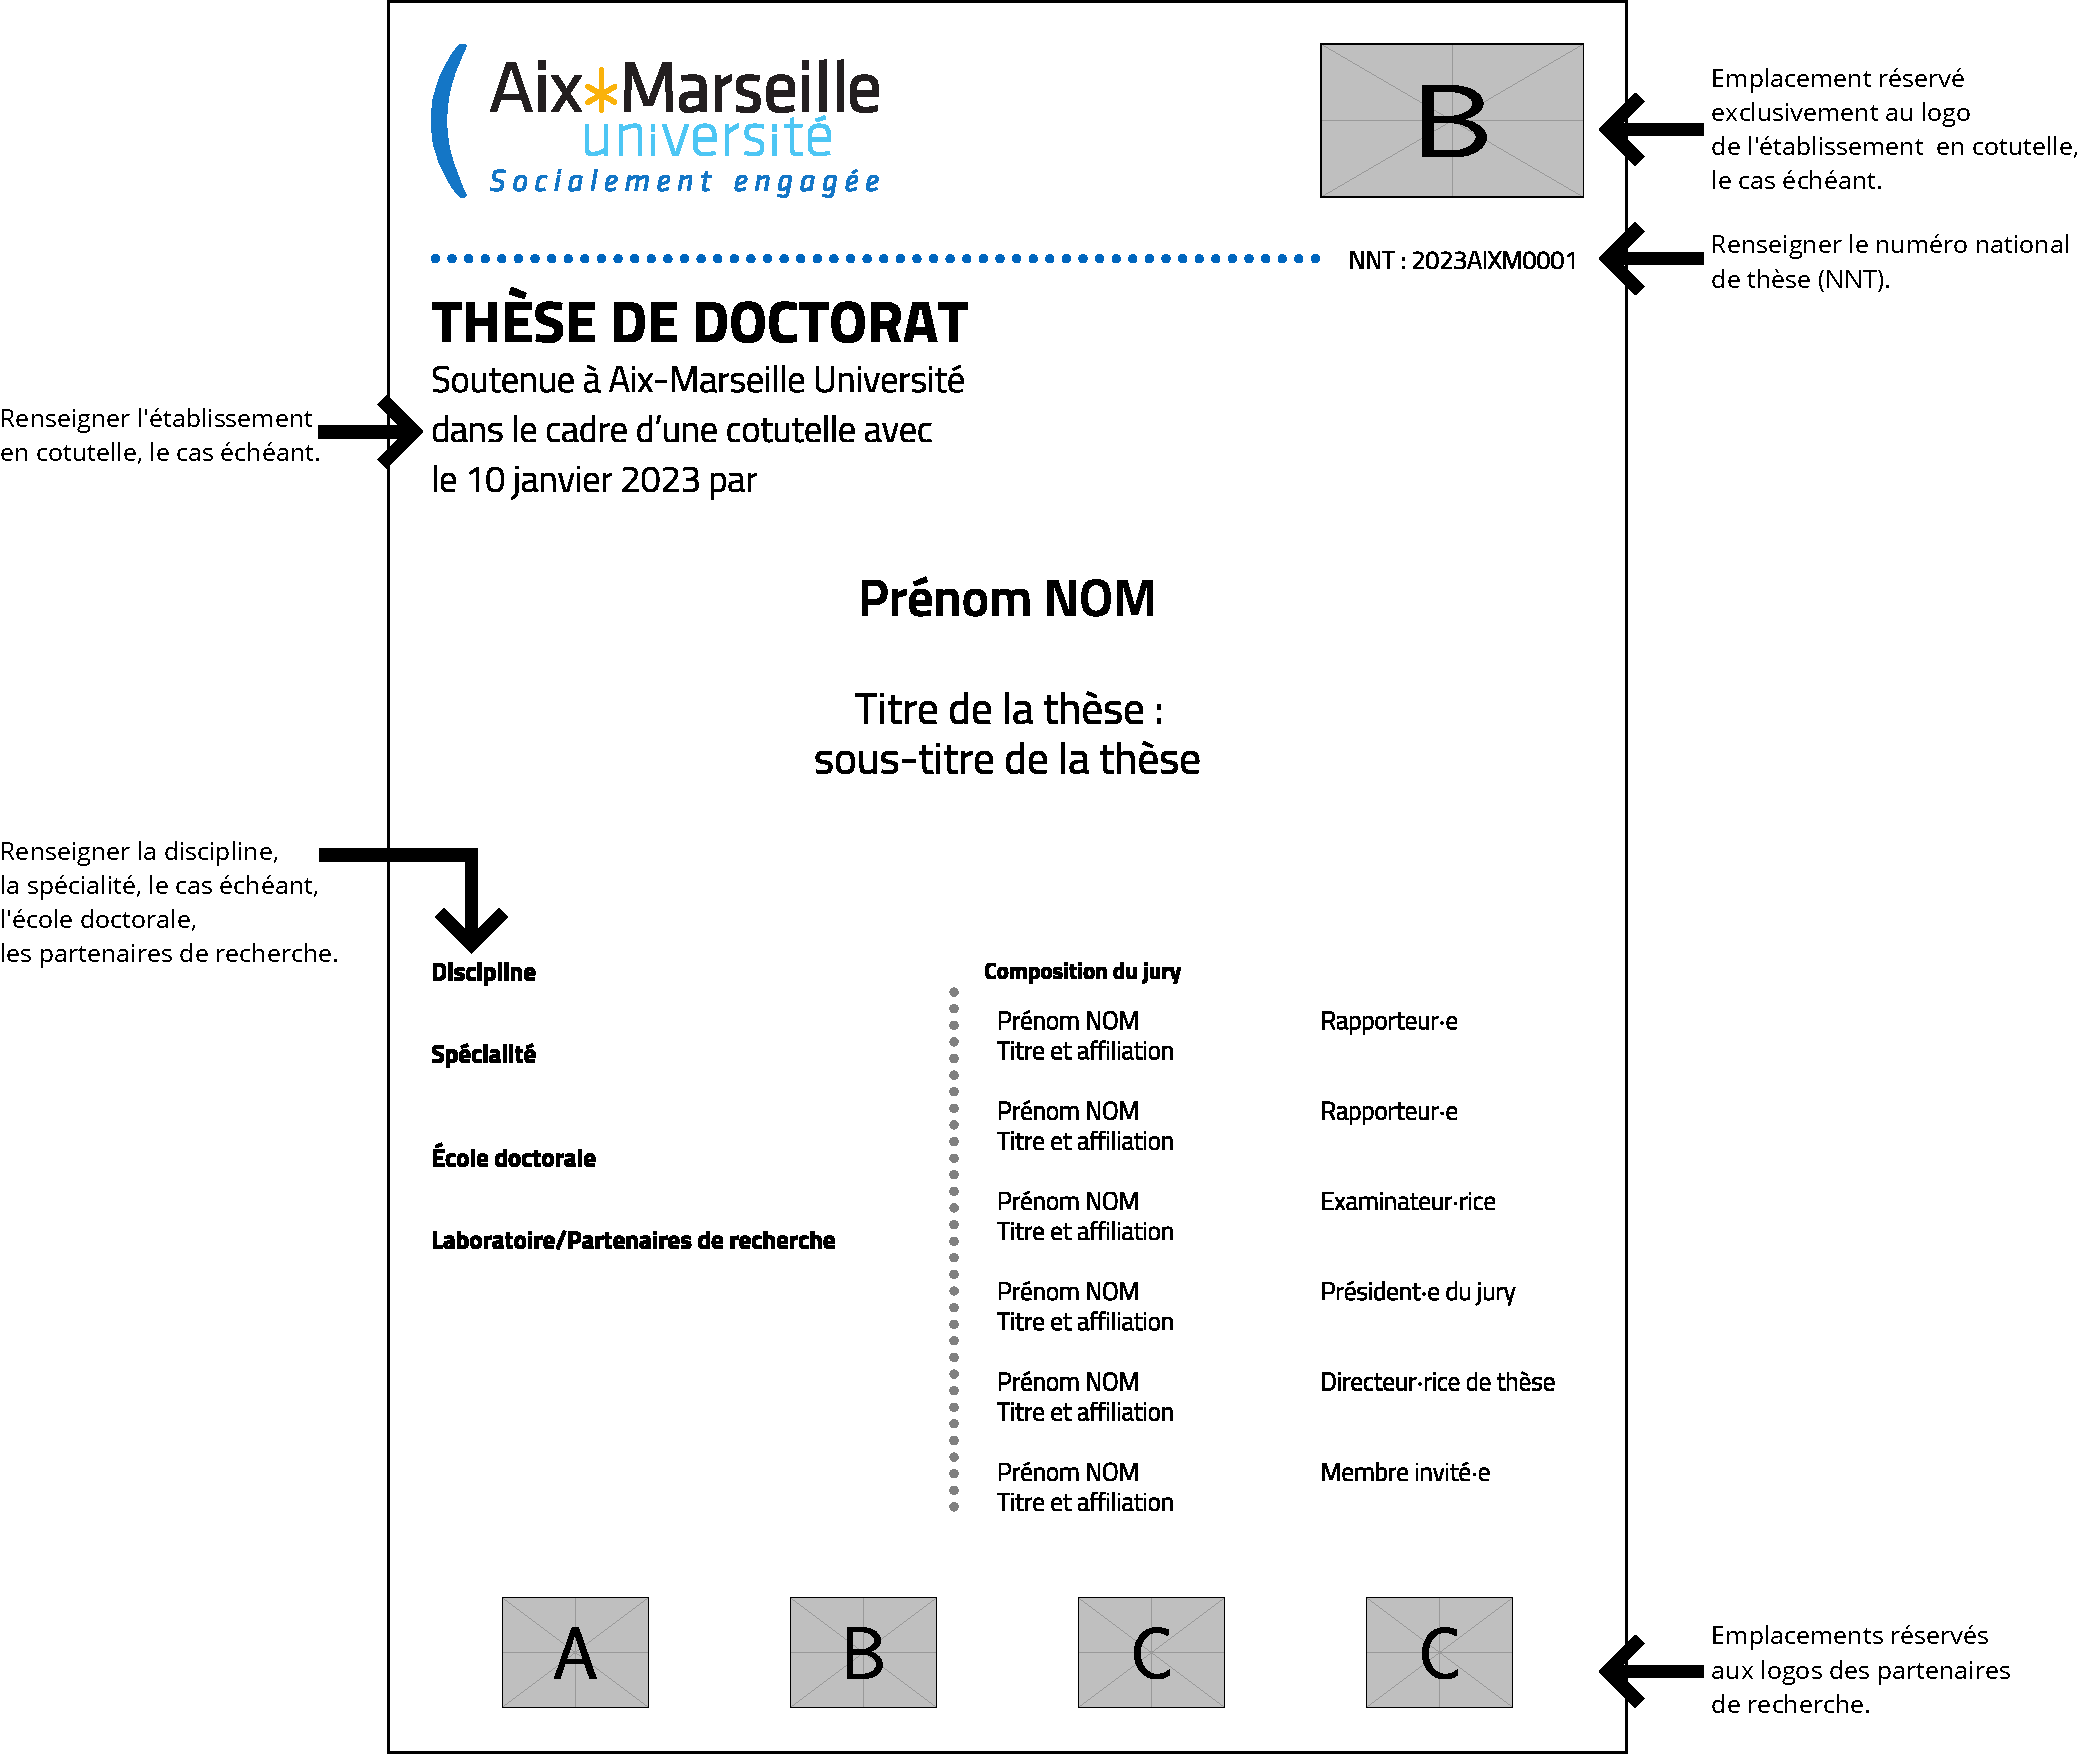
\includegraphics[width=0.8\textwidth]{titre.pdf}
\end{figure}

\begin{enumerate}
    \item The title page of AMU’s thesis: it is written in French with the Titillium font, provided with the LaTeX AMU template in TTF and TFM formats, according to AMU’s graphic charter.
    \item In the case of international cotutelle, the logo of the partner institution must appear at the top right of the title page;
	\item The composition of the jury, the doctoral school, the discipline and the specialty (if applicable) must be in accordance with the ADUM application form for the thesis defense;
	\item The national thesis number (NNT) must be displayed on the title page;
	\item Where appropriate, logos of partner institutions or research units can be added to the bottom of the title page;
	\item The \nameref{chap:affidavit} page: according to the language used for writing your thesis, choose the French or English version, then complete, date and sign it;
	\item The \nameref{chap:publications} page made during the course of your thesis project ;
	\item \nameref{chap:resume} in French and \nameref{chap:abstract} in English pages: each summary must not exceed 4,000 characters.\\
\end{enumerate}

Depending on your needs, you can add the following elements: summary and/or table of contents, list of figures, list of tables, list of acronyms, glossary, index, nomenclature...
For the body of your thesis, if your doctoral school does not give you more specific instructions, you can use the styles established in this template or your own styles following these recommendations:
\begin{itemize}
	\item Neutral font : It is recommended to use a standard serif font for text and a standard sans-serif font for titles;
	\item Geometry : paper=a4, fontsize=12pt, DIV=12;
	\item Single-line spacing;
	\item Justified text.\\
\end{itemize}

\begin{figure}[h!tbp]
	%\vspace{0.5cm}
	\centering
	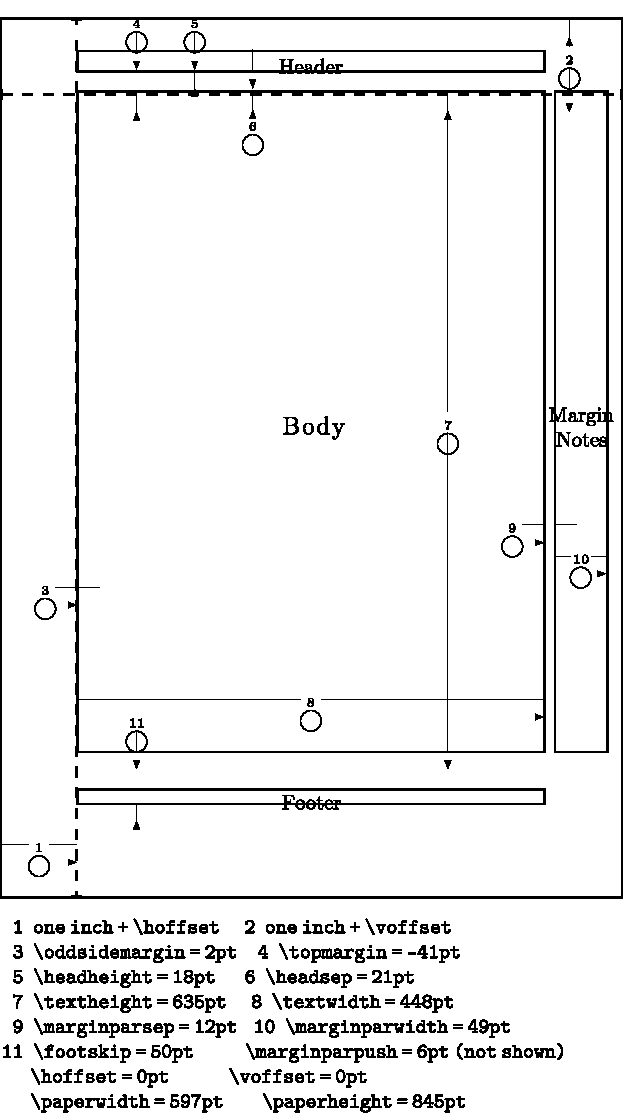
\includegraphics[width=0.3\textwidth]{geometry.pdf}
\end{figure}

Your thesis must be submitted online in PDF 1.5 minimum version format on \href{https://www.adum.fr/}{adum.fr}.

\selectlanguage{french}
			%% annexes

\end{document}
